\chapter{Metodologia}\label{metodologia}
Com o objetivo de apresentar os aspectos metodológicos e teóricos desta tese, optou-se por organizar este capítulo em seções que se inter-relacionam para fornecer a descrição dos modelos, das detecção de bordas e das abordagens para a fusão das evidências de bordas. 
\section{Modelagem estatística para dados PolSAR}\label{cap_model_estatistica}
%%% ACF Diga logo em qual texto você se baseou para escrever esta parte
%%% AAB Realizado
Os conceitos apresentados nesta seção são baseado nos artigos \citet{ade} e \citet{fnc2011}, assim como no livro \citet{lp}.

Os sistemas PolSAR transmitem pulsos de micro-ondas polarizados ortogonalmente e medem componentes ortogonais do sinal recebido. Para cada pixel, a medida resulta em uma matriz de coeficientes de espalhamento. Esses coeficientes são números complexos que descrevem no sistema SAR a transformação do campo eletromagnético transmitido para o campo eletromagnético recebido.

%%% ACF Eu gosto mais do espaçamento que se obtem usando \bmatrix do pacote amsmath. Veja o que acha:
%%% AAB realizado - concordei, simplifica notação tb 
A transformação pode ser representada como
\begin{equation*}
\begin{bmatrix}
	E_\text{h}^\text{r}   \\
	E_\text{v}^\text{r}    \\
\end{bmatrix}
 = \frac{e^{\hat{\imath} \text{kd}}}{\text{d}}
\begin{bmatrix}
	S_{\text{hh}}   & S_{\text{hv}}   \\
	S_{\text{vh}}   & S_{\text{vv}}   \\
\end{bmatrix}
\begin{bmatrix}
	E_\text{h}^\text{t}   \\
	E_\text{v}^\text{t}   \\
\end{bmatrix},
\end{equation*}
onde k denota o número de onda, $\hat{\imath}$ é um número complexo e d é a distância entre o radar e o alvo. No campo eletromagnético com componentes $E_\text{i}^\text{j}$, o índice subscrito denota polarização horizontal (h) ou vertical (v), e o índice sobrescrito indica a onda recebida (r) ou transmitida (t). 

A matriz de espalhamento complexa $\mathbf{S}$ é definida por
\begin{equation}
\mathbf{S} = 
\begin{bmatrix}
	S_\text{hh}   & S_\text{hv}   \\
	S_\text{vh}   & S_\text{vv}   \\
\end{bmatrix},
\label{matriz_de_espalhamento}
\end{equation}
\index{Matriz de Espalhamento}
onde as entradas da matriz $S_\text{i,j}$ são os coeficientes de espalhamento complexos, tal que os índices i e j são associados ao  recebimento e a transmissão das ondas, por exemplo, o coeficiente de espalhamento $S_\text{hv}$ está associado a onda transmitida na direção vertical (v) e recebida na direção horizontal (h).

%%% ACF Escreva esse parágrafo de forma direta, se necessário em mais de uma frase
%%% AAB realizado
A co-polarização é definida pela relação entre os elementos da diagonal principal. E a polarização cruzada é a relação entre os elementos da diagonal secundária. 

A potência total espalhada no caso de um sistema de radar polarimétrico é o chamado \textit{Span}, sendo definido no caso geral como:
\begin{equation}
\mathit{Span}(\mathbf{S}) = \traco(\mathbf{S}\mathbf{S}^\text{H})=|S_\text{hh}|^2+|S_\text{hv}|^2+|S_\text{vh}|^2+|S_\text{vv}|^2,
\label{span_geral}
\end{equation}
\index{Span}
onde o operador $\traco(\cdot)$ é o traço de uma matriz, e o superíndice H denota a matriz transposta conjugada.
\subsection{Matriz de coerência polarimétrica de Pauli ($\mathbf{T}_4$) e matriz de covariância lexicográfica ($\mathbf{C}_4$)}
A matriz de espalhamento $\mathbf{S}$ pode ser representada pela construção do vetor
\begin{equation}
\mathbf{k}=\frac{1}{2}\left[\traco(\mathbf{S}\Psi_1)\quad\traco(\mathbf{S}\Psi_2)\quad \traco(\mathbf{S}\Psi_3)\quad \traco(\mathbf{S}\Psi_4)\right]^T,
\label{def_vet_espalhamento_4d}
\end{equation}
onde $\{\Psi_i\}_{i=1}^4$ é uma base para o espaço das matrizes hermitianas $2\times 2$.

Diferentes bases para o mesmo espaço das matrizes podem ser definidas.
Vamos escolher duas bases, a primeira chamada de  base de Pauli, ver \citep{lp}:
%%% ACF Os "labels" de equações devem ir no final, caso contrário pode bagunçar a numeração. Revise tudo.
%%% AAB OK
\begin{equation}
\{\Psi_P\} = \left\{
\sqrt{2}\begin{bmatrix}
	1  & 0  \\
	0  & 1 \\
\end{bmatrix},
\sqrt{2}\begin{bmatrix}
	1  & 0  \\
	0  & -1  \\
\end{bmatrix},
\sqrt{2}\begin{bmatrix}
	0  & 1  \\
	1  & 0  \\
\end{bmatrix},
\sqrt{2}\begin{bmatrix}
	0       & -\hat\imath  \\
	\hat\imath  & 0  \\
\end{bmatrix}
\right\},
\label{base_de_pauli_4d}
\end{equation}
\index{Base de Pauli de dimensão 4}
e a segunda chamada de base lexicográfica, ver \citep{lp}:
\begin{equation}
\{\Psi_L\} = \left\{
2\begin{bmatrix}
	1  & 0  \\
	0  & 0 \\
\end{bmatrix},
2\begin{bmatrix}
	0  & 1  \\
	0  & 0  \\
\end{bmatrix},
2\begin{bmatrix}
	0  & 0  \\
	1  & 0 \\
\end{bmatrix},
2\begin{bmatrix}
	0  & 0  \\
	0  & 1  \\
\end{bmatrix}
\right\}.
\label{base_lexicografica_4d}
\end{equation}
\index{Base Lexicográfica de dimensão 4}

Sendo o vetor \eqref{def_vet_espalhamento_4d}, e usando a base \eqref{base_de_pauli_4d} representamos a matriz de espalhamento pelo vetor característico de Pauli $4$-D,
\begin{equation}
\mathbf{k}= \frac{1}{\sqrt{2}}
	\begin{bmatrix}
	S_\text{hh} + S_\text{vv}& S_\text{hh} - S_\text{vv}& S_\text{hv} + S_\text{vh} &\hat\imath(S_\text{hv} - S_\text{vh})   \\
\end{bmatrix}^\text{T}=\frac{1}{\sqrt{2}}[k_1\quad k_2\quad k_3\quad k_4]^\text{T},
\label{vetor_pauli_4d}
\end{equation}
e usando a base \eqref{base_lexicografica_4d} representamos a matriz de espalhamento pelo vetor característico lexicográfico $4$-D, 
\begin{equation}
\mathbf{\Omega}=
	\begin{bmatrix}
	S_\text{hh}& S_\text{hv} &S_\text{hv}& S_\text{vv}   \\
\end{bmatrix}^\text{T}=[\Omega_1\quad \Omega_2\quad \Omega_3\quad \Omega_4]^\text{T}.
\label{vetor_lexicografico_4d}
\end{equation}

A matriz de espalhamento pode ser relacionada com os vetores \eqref{vetor_pauli_4d} e \eqref{vetor_lexicografico_4d} da seguinte maneira,
\begin{equation}
\mathbf{S} = 
\begin{bmatrix}
	S_\text{hh}   & S_\text{hv}   \\
	S_\text{vh}   & S_\text{vv}   \\
\end{bmatrix}
=
\begin{bmatrix}
	\Omega_1   & \Omega_2   \\
	\Omega_3   & \Omega_4   \\
\end{bmatrix}
=\frac{1}{\sqrt{2}}
\begin{bmatrix}
	 k_1+k_2  & k_3-\hat\imath k_4   \\
	 k_3+\hat\imath k_4 & k_1-k_2   \\
\end{bmatrix}
\label{mat_esp_rel_pauli_lex}
\end{equation}

As constantes $2$ e $\sqrt{2}$ nas bases \eqref{base_de_pauli_4d} e \eqref{base_lexicografica_4d} ajustam a norma dos vetores de espalhamento para serem iguais, independente da escolha das bases. O produto interno escolhido é o padrão para o espaço vetorial dos vetores complexos de dimensão 4, isto é, se $\mathbf{u}$ e $\mathbf{v}$ são vetores complexos, o produto interno é $\mathbf{u}^\text{H}\mathbf{v}$.

%%% ACF A seguinte equação fica com melhor espaçamento usando "align"
%%% AAB Realizado
Podemos assim garantir a invariância do \textit{Span}:
\begin{align}\nonumber
\mathit{Span}(\mathbf{S}) &=\traco(\mathbf{S}\mathbf{S}^\text{H})=|S_\text{hh}|^2+|S_\text{hv}|^2+|S_\text{vh}|^2+|S_\text{vv}|^2  \\\nonumber
	   &=  \mathbf{k}^\text{H}\mathbf{k}=|\mathbf{k}|^2\\
	   &=\mathbf{\Omega}^\text{H}\mathbf{\Omega} =|\mathbf{\Omega}|^2.\\\nonumber
\label{span_invariante}
\end{align}

A matriz unitária $\mathbf{U}_4$ é a representação matricial da transformação linear que aplica o vetor na base lexicográfica em um vetor na base de Pauli. 
Podemos gerar a  matriz unitária colocando nas linhas da matriz os elementos da base de Pauli:
\begin{equation}
\mathbf{U}_4=	\frac{1}{\sqrt{2}}	
\begin{bmatrix}
	1   & 0 & 0 & 1  \\
	1   & 0 & 0 & -1  \\
	0   & 1 & 1 & 0  \\
	0   & \hat\imath & -\hat\imath &0   \\
\end{bmatrix}.
\label{matriz_unit_su4}
\end{equation}

A transformação linear $\mathbf{k}=\mathbf{U}_4\mathbf{\Omega}$, representada em forma matricial
\begin{equation}
\frac{1}{\sqrt{2}}
\begin{bmatrix}
	  S_\text{hh} +  S_\text{vv}\\  
	  S_\text{hh} -  S_\text{vv}\\
	  S_\text{hv} +  S_\text{vh} \\
        \hat\imath(S_\text{hv} -  S_\text{vh}) \\
\end{bmatrix}
=\frac{1}{\sqrt{2}}	
\begin{bmatrix}
	1   & 0 & 0 & 1  \\
	1   & 0 & 0 & -1  \\
	0   & 1 & 1 & 0  \\
	0   & \hat\imath & -\hat\imath &0   \\
\end{bmatrix}
\begin{bmatrix}
	S_\text{hh} \\  
	S_\text{hv} \\
	S_\text{vh} \\
	S_\text{vv} \\
\end{bmatrix}
\label{trans_matriz_unit_su4}
\end{equation}
foi definida para demonstrar a transformação similar entre a matriz de coerência, e a matriz de covariância definidas a seguir.  

A matriz de coerência polarimétrica de Pauli é definida por,  
\begin{equation}
	\mathbf{T}_4=\mathbf{k}\mathbf{k}^\text{H}=	
\begin{bmatrix}
	|k_1|^2       & k_1\bar{k}_2  & k_1\bar{k}_3  & k_1\bar{k}_4  \\
	k_2\bar{k}_1  & |k_2|^2       & k_2\bar{k}_3  & k_2\bar{k}_4  \\
	k_3\bar{k}_1  & k_3\bar{k}_2  &    |k_3|^2    & k_3\bar{k}_4  \\
	k_4\bar{k}_1  & k_4\bar{k}_2  & k_4\bar{k}_3  & |k_4|^2   \\
\end{bmatrix}
\label{matriz_polar_pauli}
\end{equation}\index{Matriz polarimétrica de Pauli $4\times 4$}
%%% ACF Definiu $\bar{k}$? 
%%% AAB Realizado
e a matriz de covariância lexicográfica
\begin{equation}
	\mathbf{C}_4=\mathbf{\Omega}\mathbf{\Omega}^\text{H}=	
\begin{bmatrix}
	|\Omega_1|^2       & \Omega_1\bar{\Omega}_2  & \Omega_1\bar{\Omega}_3  & \Omega_1\bar{\Omega}_4  \\
	\Omega_2\bar{\Omega}_1  & |\Omega_2|^2       & \Omega_2\bar{\Omega}_3  & \Omega_2\bar{\Omega}_4  \\
	\Omega_3\bar{\Omega}_1  & \Omega_3\bar{\Omega}_2  &    |\Omega_3|^2    & \Omega_3\bar{\Omega}_4  \\
	\Omega_4\bar{\Omega}_1  & \Omega_4\bar{\Omega}_2  & \Omega_4\bar{\Omega}_3  & |\Omega_4|^2   \\
\end{bmatrix},
\label{matriz_covar_lexic}
\end{equation}\index{Matriz de covariância lexicográfica $4\times 4$}
onde, $\bar{k}$ e $\bar{\Omega}$ são, respectivamente, os conjugados dos números complexos $k$ e $\Omega$.

As matrizes de coerência polarimétrica de Pauli e covariância lexicográfica são relacionadas usando as definições e a propriedade \eqref{trans_matriz_unit_su4}, assim teremos:
$$
	\mathbf{T}_4=\mathbf{k}\mathbf{k}^\text{H} =\mathbf{U}_4\mathbf{\Omega}(\mathbf{U_4\Omega})^H	
	           =\mathbf{U_4\Omega}\mathbf{\Omega}^H\mathbf{U_4}^H =\mathbf{U_4}\mathbf{C}_4\mathbf{U_4}^H	
$$
então, a relação de similaridade entre as matrizes é,
\begin{align}
\mathbf{T}_4  &=\mathbf{U_4}\mathbf{C}_4\mathbf{U_4}^\text{H}\\
\label{matriz_simil_t4_c4}\nonumber
\end{align}
lembrando que $\mathbf{U_4}$ é unitária, e o traço é a soma dos autovalores de uma matriz, concluímos:
\begin{equation}
	\traco({\mathbf{T}_4})  =\traco({\mathbf{C}_4})=\mathit{Span}\mathbf{(S)}.\\
\label{traco_t4_c4}
\end{equation}
\subsection{Matriz de coerência polarimétrica de Pauli ($\mathbf{T}_3$) e matriz de covariância lexicográfica ($\mathbf{C}_3$)}
Podemos entender as interações das ondas eletromagnéticas em alvos naturais sob a ótica do teorema da reciprocidade, o qual considera que o meio é recíproco. 
De uma maneira geral as propriedades de transmissão e recebimento de uma antena são idênticos, e mono-estáticos, ou seja, consideramos o sistema de coordenada BSA - \textit{Back Scattering Alignment}. 
Em meios recíprocos podemos definir a igualdade dos termos de polarização cruzada $S_\text{hv}=S_\text{vh}$; ver \citet{lp}. 

A matriz de espalhamento $\mathbf{S}$ pode ser representada pelo vetor
\begin{equation}
\mathbf{k}=\frac{1}{2}\left[\traco(S\Psi_1)\quad\traco(S\Psi_2)\quad \traco(S\Psi_3)\right]^T,
\label{def_vet_espalhamento_3d}
\end{equation}
onde $\{\Psi_i\}_{i=1}^3$ é uma base para o espaço das matrizes hermitianas $2\times 2$.

%%% ACF Aqui faça uma transição. Deixe claro que as bases lexicográfica e de Pauli vistas antes são 4D, e que aqui as veremos para 3D. Evite que pareça copiar-colar
%%% AAB Realizado
Em meios recíprocos a matriz de espalhamento é hermitiana, portanto o vetor de espalhamento 4-D, a matriz de coerência polarimétrica de Pauli $\mathbf{T}_4$  e a matriz de covariância lexicográfica $\mathbf{C}_4$ são reduzidas para o vetor de espalhamento 3-D, a matriz de coerência polarimétrica de Pauli $\mathbf{T}_3$  e a matriz de covariância lexicográfica $\mathbf{C}_3$, com as ferramentas desenvolvidas nesta seção.

Diferentes bases para o mesmo espaço das matrizes podem ser definidas, vamos escolher duas bases, a primeira chamada base de Pauli:
\begin{equation}
\{\Psi_P\} = \left\{
\sqrt{2}\begin{bmatrix}
	1  & 0  \\
	0  & 1 \\
\end{bmatrix},
\sqrt{2}\begin{bmatrix}
	1  & 0  \\
	0  & -1  \\
\end{bmatrix},
\sqrt{2}\begin{bmatrix}
	0  & 1  \\
	1  & 0  \\
\end{bmatrix}
\right\},
\label{base_de_pauli_3d}
\end{equation}\index{Base de Pauli de dimensão 3}
e a segunda chamada base lexicográfica:
\begin{equation}
\{\Psi_L\} = \left\{
2\begin{bmatrix}
	1  & 0  \\
	0  & 0 \\
\end{bmatrix},
2\sqrt{2}\begin{bmatrix}
	0  & 1  \\
	0  & 0  \\
\end{bmatrix},
2\begin{bmatrix}
	0  & 0  \\
	0  & 1  \\
\end{bmatrix}
\right\}.
\label{base_lexicografica_3d}
\end{equation}\index{Base lexicográfica de dimensão 3}

Sendo o vetor \eqref{def_vet_espalhamento_3d}, e usando a base \eqref{base_de_pauli_3d} representamos a matriz de espalhamento pelo vetor característico de Pauli $3$-D,
\begin{equation}
\mathbf{k}= \frac{1}{\sqrt{2}}
	\begin{bmatrix}
	S_\text{hh} + S_\text{vv} & S_\text{hh} - S_\text{vv}& 2S_\text{hv}   \\
\end{bmatrix}^\text{T}=\frac{1}{\sqrt{2}}[k_1\quad k_2\quad k_3]^\text{T},
\label{vetor_pauli_3d}
\end{equation}
e usando a base \eqref{base_lexicografica_3d} representamos a matriz de espalhamento pelo vetor característico lexicográfico $3$-D,  
\begin{equation}
\mathbf{\Omega}= \frac{1}{\sqrt{2}}
	\begin{bmatrix}
	S_\text{hh}& S_\text{hv}& S_\text{vv}   \\
\end{bmatrix}^\text{T}=[\Omega_1\quad \Omega_2\quad \Omega_3]^\text{T}.
\label{vetor_lexicografico_3d}
\end{equation}

As constantes $2$ e $\sqrt{2}$ nas bases \eqref{base_de_pauli_3d} e \eqref{base_lexicografica_3d} servem para manter a norma dos vetores de espalhamento iguais, independente da escolha das bases. O produto interno escolhido é o padrão para o espaço vetorial dos vetores complexos de dimensão 3, isto é, se $\mathbf{u}$ e $\mathbf{v}$ são vetores complexos, o produto interno é $\mathbf{u}^\text{H}\mathbf{v}$.

Podemos assim garantir a invariância da potência total,
\begin{align}\nonumber
\mathit{Span}(\mathbf{S}) &=  \traco(\mathbf{SS}^\text{H})=|S_{hh}|^2+2|S_{hv}|^2+|S_{vv}|^2  \\\nonumber
	   &=  \mathbf{k}^\text{H}\mathbf{k}=|\mathbf{k}|^2\\
	   &=  \mathbf{\Omega}^\text{H}\mathbf{\Omega}=|\mathbf{\Omega}|^2\\\nonumber
\label{span_invariante_3d}
\end{align}

A matriz unitária $\mathbf{U}_3$ é definida como a representação matricial da transformação linear que aplica o vetor na base lexicográfica em um vetor na base de Pauli. Podemos gerar a  matriz unitária colocando nas linhas da matriz os elementos da base de Pauli, portanto,
\begin{equation}
\mathbf{U}_3=\frac{1}{\sqrt{2}}	
\begin{bmatrix}
	1   & 0 & 1  \\
	1   & 0 & -1  \\
	0   & \sqrt{2} &  0  \\
\end{bmatrix}.
\label{matriz_unit_su3}
\end{equation}

A transformação linear $\mathbf{k}=\mathbf{U}_3\mathbf{\Omega}$, representado na forma matricial,
\begin{equation}
\frac{1}{\sqrt{2}}
\begin{bmatrix}
	  S_\text{hh} +  S_\text{vv}\\  
	  S_\text{hh} -  S_\text{vv}\\
	  2  S_\text{hv} \\
\end{bmatrix}
=\frac{1}{\sqrt{2}}	
\begin{bmatrix}
	1   & 0 & 1  \\
	1   & 0 & -1  \\
	0   & 2 &  0  \\
\end{bmatrix}
\begin{bmatrix}
	S_\text{hh} \\  
	S_\text{hv} \\
	S_\text{vv}\\
\end{bmatrix}
\label{trans_matriz_unit_su3}
\end{equation}
foi definida para demonstrar a transformação similar entre a matriz de coerência, e a matriz de covariância definidas a seguir.

A matriz de coerência polarimétrica de Pauli é definida por,
\begin{equation}
	\mathbf{T}_3=\mathbf{k}\mathbf{k}^\text{H}=	
\begin{bmatrix}
	|k_1|^2       & k_1\bar{k}_2  & k_1\bar{k}_3  \\
	k_2\bar{k}_1  & |k_2|^2       & k_2\bar{k}_3  \\
	k_3\bar{k}_1  & k_3\bar{k}_2  &    |k_3|^2    \\
\end{bmatrix}
\label{matriz_polar_pauli_3}
\end{equation}\index{Matriz polarimétrica de Pauli $3\times 3$}
e a matriz de covariância lexicográfica
\begin{equation}
	\mathbf{C}_3=\mathbf{\Omega}\mathbf{\Omega}^\text{H}=	
\begin{bmatrix}
	|\Omega_1|^2       & \Omega_1\bar{\Omega}_2  & \Omega_1\bar{\Omega}_3   \\
	\Omega_2\bar{\Omega}_1  & |\Omega_2|^2       & \Omega_2\bar{\Omega}_3  \\
	\Omega_3\bar{\Omega}_1  & \Omega_3\bar{\Omega}_2  &    |\Omega_3|^2      \\
\end{bmatrix},
\label{matriz_covar_lexic_3}
\end{equation}\index{Matriz de covariância polarimétrica $3\times 3$}
onde, $\bar{k}$ e $\bar{\Omega}$ são, respectivamente, os conjugados dos números complexos $k$ e $\Omega$.

As matrizes de coerência polarimétrica de Pauli e covariância lexicográfica são relacionadas usando as definições e a propriedade \eqref{trans_matriz_unit_su4}, assim teremos
$$
	\mathbf{T}_3=\mathbf{k}\mathbf{k}^\text{H}=\mathbf{U_3\Omega}(\mathbf{U_3\Omega})^\text{H}	\\
	=\mathbf{U_3\Omega}\mathbf{\Omega}^\text{H}\mathbf{U_3}^\text{H}=\mathbf{U_3}\mathbf{C}_3\mathbf{U_3}^\text{H},
$$
então, a relação de similaridade entre as matrizes é,
\begin{equation}
	 \mathbf{T}_3  =\mathbf{U_3}\mathbf{C}_3\mathbf{U_3}^\text{H}\\
\label{matriz_simil_t3_c3}
\end{equation}
lembrando que $\mathbf{U_3}$ é unitária, e o traço é a soma dos autovalores de uma matriz, concluímos
\begin{equation}
	\traco({\mathbf{T}_3})  =\traco({\mathbf{C}_3})=\mathit{Span}\mathbf{(S)}.\\
\label{traco_t3_c3}
\end{equation}

Portanto podemos afirmar, se
\begin{equation} 
\mathbf{s} = 
\begin{bmatrix}
	S_\text{hh}      \\
        \sqrt{2}S_\text{hv}     \\
	S_\text{vv}      \\
\end{bmatrix},
\label{vetor_3d}
\end{equation}
a potência total espalhada, no caso de um sistema de radar polarimétrico em meio recíproco, é:
\begin{equation}
\mathit{Span} = \traco(\mathbf{SS}^\text{H})=|S_\text{hh}|^2+2|S_\text{hv}|^2+|S_\text{vv}|^2.
\label{span_geral}
\end{equation}
\subsection{Estatística do Ruído \textit{Speckle} no processo de única visada}\index{O ruído \textit{Speckle}}
As imagens SAR e PolSAR possuem um tipo de ruído multiplicativo chamado \textit{speckle}, conhecido por causar variação de intensidade pixel a pixel, que lhes imprime um aspecto granular.  

O \textit{speckle} dificulta a interpretação e análise das imagens reduzindo a efetividade da segmentação, classificação, ou detecção de mudanças de características das imagens SAR e PolSAR. O entendimento do comportamento estatístico do \textit{speckle} é essencial para extrair boas informações das imagens e propor algoritmos efetivos para tratar esse tipo de ruído. 

Neste trabalho usaremos as características do ruído \textit{speckle} para auxiliar na detecção de borda, em oposição a trabalhos que tentam mitigar o efeito do ruído.

%%% ACF O speckle é inerente a todo tipo de iluminação coerente. 
%%% AAB realizado  
O \textit{speckle} é inerente ao processo do radar iluminar uma superfície rugosa, como florestas, plantações, áreas urbanas, e etc, então o sinal de retorno consiste em ondas refletidas com muitos elementos de espalhamento. Os elementos de espalhamento têm geometrias complexas e distribuições aleatórias, tornando a modelagem estatística uma tarefa indispensável e desafiadora. 

Podemos considerar três tipos de processos de espalhamento da onda em alvos (elementos de espalhamento): dispersão de superfície, dispersão de volume, e o espalhamento de volume-superfície. 
O primeiro é o espalhamento que acontece quando a onda eletromagnética atravessa uma mudança de meio de propagação. 
O segundo consiste no espalhamento que acontece na profundidade de um meio, por exemplo, o espalhamento no interior de uma floresta. 
Por último, o espalhamento volume-superfície consiste em a onda atingir outro meio de propagação, por exemplo o solo de uma floresta.
 
As distância entre os elementos de espalhamento e o recebimento no radar varia devido a natureza randômica da disposição desses elementos. 
As ondas recebidas de cada elemento espalhador, embora coerentes em frequência, não são coerentes em fase. Assim, podemos considerar o sinal é forte se as ondas são construtivas, ou seja em fase, e fraco se a ondas não estão em fase, ou seja se estão espalhadas de forma destrutiva.
 
Podemos escrever um sinal complexo da seguinte forma:
\begin{equation}
\sum_{i=1}^{M}(x_i+\hat{\jmath} y_i)=\sum_{i=1}^{M}x_i+\hat{\jmath}\sum_{i=1}^{M} y_i=x+\hat{\jmath} y=r\exp(\hat{\jmath}\theta),
\label{eq:speckle_soma}
\end{equation}
onde $x_i+\hat{\jmath} y_i$ é o retorno do espalhamento para cada elemento $i$.
Se o sinal é resultante da interação de $M$ elementos espalhadores, então $x+\hat{\jmath}y$ é a soma destes elementos, e $r\exp(\hat{\jmath}\theta)$ é a decomposição de Euler para o número complexo $x+\hat{\jmath}y$.
\subsubsection{Modelo de Rayleigh para o \textit{speckle}}
Definir um modelo para o \textit{speckle} é muito importante na tarefa de obter informação de imagens SAR e PolSAR. 
Com esse objetivo, estipulamos as seguintes condições para a modelagem de áreas homogêneas:
\begin{itemize}
\item Há um número muito grande de espalhadores na célula de resolução.
\item A distância entre eles é muito menor que o comprimento de onda do radar.
\item A superfície tem maior rugosidade na escala do comprimento de onda de um radar.
\end{itemize}
Os trabalhos de \citet{AGeneralizedGaussianCoherentScattererModelforCorrelatedSARTexture,SARImageStatisticalModelingPartISinglePixelStatisticalModels} fazem uma análise detalhada dessas e de outras condições, bem como das distribuições resultantes.

O \textit{speckle} totalmente desenvolvido é definido utilizando o vetor soma \eqref{eq:speckle_soma} para os retornos dos espalhamentos de alvos de forma que a sua fase seja distribuída uniformemente no intervalo $(-\pi,\pi)$. 

O teorema central do limite para o \textit{speckle} totalmente desenvolvido garante que as componentes $x$ e $y$ sejam gaussianas, independentes e identicamente distribuídas com média zero e variância $\frac{\sigma^2}{2}$. 
A sua função densidade de probabilidade conjunta é dada por
\begin{equation}
\begin{split}
  f_{XY}(x,y;\sigma^2)&=f_X(x;\sigma^2)f_Y(y;\sigma^2)\\
  &=\frac{1}{\sqrt{\pi}\sigma}\exp\left(-\frac{x^2}{\sigma^2}\right)\frac{1}{\sqrt{\pi}\sigma}\exp\left(-\frac{y^2}{\sigma^2}\right)=\frac{1}{\pi\sigma^2}\exp\left(-\frac{x^2+y^2}{\sigma^2}\right).
 \end{split}
 \label{eq:pdf_gaussiana_xy}
 \end{equation}
Fazendo $x=z_A\cos\theta$, e $y=z_A\sin\theta$ teremos
\begin{equation}
f_{A}(z_A;\sigma^2)=\frac{z_A}{\pi\sigma^2}\exp\left(-\frac{z_A^2(\cos^2\theta+\sin^2\theta)}{\sigma^2}\right)=\frac{z_A}{\pi\sigma^2}\exp\left(-\frac{z_A^2}{\sigma^2}\right).
\label{eq:pdf_gaussiana_Atheta}
\end{equation}

Integrando na variável $\theta$ no intervalo de $(-\pi,\pi)$ encontramos a distribuição para a amplitude.
\begin{equation}\nonumber
f_A(z_A;\sigma^2)=\int_{-\pi}^{\pi}\frac{z_A}{\pi\sigma^2}\exp\left(-\frac{z_A^2}{\sigma^2}\right)d\theta=\frac{z_A}{\pi\sigma^2}\exp\left(-\frac{z_A^2}{\sigma^2}\right)\int_{-\pi}^{\pi}d\theta,
\end{equation}
que é a distribuição Rayleigh, caracterizada pela função de densidade de probabilidade
\begin{equation}\nonumber
f_A(z_A;\sigma^2)=\frac{2z_A}{\sigma^2}\exp\left(-\frac{z_A^2}{\sigma^2}\right).
\end{equation}

Podemos encontrar o valor esperado ou média
\begin{equation}\nonumber
\text{M}(z_A)=E[z_A]=\int_0^\infty z_Af(z_A)dA=\int_0^	\infty \frac{2z_A^2}{\sigma^2}\exp\left(-\frac{z_A^2}{\sigma^2}\right) dz_A=\frac{\sqrt{\pi}\sigma}{2},
\end{equation} 
e
\begin{equation}\nonumber
E[z_A^2]=\int_0^\infty z_A^2f(z_A)dA=\int_0^	\infty \frac{2z_A^3}{\sigma^2}\exp\left(-\frac{z_A^2}{\sigma^2}\right) dA=\sigma^2,
\end{equation}
com o objetivo de calcular a variância
\begin{equation}\nonumber
\text{var}=E[z_A^2]-E[z_A]^2=\sigma^2-\left(\frac{\sqrt{\pi}\sigma}{2}\right)^2=\sigma^2-\frac{\pi\sigma^2}{4}.
\end{equation}

O coeficiente de variação é calculado pela razão entre o desvio padrão e a média, portanto: 
\begin{equation}
\text{CV}(Z_A) =\frac{\sqrt{\text{var}}}{\text{M}(z_A)}=\frac{\sqrt{\sigma^2-\frac{\pi\sigma^2}{4}}}{\frac{\sqrt{\pi}\sigma}{2}}=\sqrt{\frac{\sigma^2-\frac{\pi\sigma^2}{4}}{\frac{\pi\sigma^2}{4}}}=\sqrt{\frac{4}{\pi}-1}=0,5227.
\label{eq:coef_var_1_visada}
\end{equation}

A intensidade é definida por $z_I=z_A^2$, então sua função densidade de probabilidade é: 
\begin{equation}
f_I(z_I;\sigma^2)=\frac{1}{\sigma^2}\exp\left(-\frac{z_I}{\sigma^2}\right),
\label{eq:DensidadeExponencial}
\end{equation}
calculando $\text{M}(z_I)=E[I]=\sigma^2$, e $E[I^2]=2\sigma^2$,  a média e a variância são respectivamente, $\text{M}(z_I)=\sigma^2$, e $\text{var}=\sigma^4$, então o coeficiente de variação  $\text{CV}(Z_I)=\frac{\sqrt{\sigma^4}}{\sigma^2}=1$. 

Comparando os valores $\text{CV}(Z_A)$ e $\text{CV}(Z_I)$ podemos afirmar que o valor do \textit{speckle} é mais pronunciado nas imagens de intensidade em relação as imagens de amplitude.
Em ambos os casos, o coeficiente de variação é constante, portanto, não é possível melhorar a relação sinal-ruído aumentando o valor médio da imagem.

\subsection{Estatística do ruído \textit{Speckle} no processo de múltiplas visadas}
O processo de redução do ruído \textit{speckle} consiste em realizar a média aritmética de vários sinais de retorno, processo conhecido por múltiplas visadas. 
O método é análogo ao de adquirir $L\geq1$ imagens e realizar a média aritmética das mesmas. 

Sob a hipótese da eq.~\eqref{eq:DensidadeExponencial} decorre que a função densidade de probabilidade para os canais de intensidades com múltiplas visadas é representado por
\begin{equation}
f_I(z_I;L,\sigma^2)=\frac{L^L z_I^{L-1}}{\Gamma(L)\sigma^{2L}}\exp\left(-L\frac{z_I}{\sigma^2}\right), z_I\geq 0,
\label{pdf_inten_multilook}
\end{equation}
onde $\Gamma(L)$ denota a função gama de Euler. Assim podemos afirmar que a intensidade com o processo de múltiplas visadas obedece uma distribuição gaussiana.

%%% ACF Aqui mudou a notação para média e variância. Não pode! Unifique!
%%% AAB Resolvido
A média e a variância são respectivamente, $\text{M}_L(z_I)=\sigma^2$, $\text{var}_L(z_I)=\frac{\sigma^4}{L}$ implicando que o desvio padrão será $\text{SD}_L(z_I)=\frac{\sigma^2}{\sqrt{L}}$. 
%%% ACF Leve a definição do CV para o local onde ele é usado pela primeira vez
%%% AAB realizado
O coeficiente de variação para o processo de múltiplas visadas em $\text{CV}_L(z_I)=\frac{1}{\sqrt{L}}$. Podemos observar que o coeficiente de variação é reduzido por $\sqrt{L}$ com relação ao processo de visada simples.

A função densidade de probabilidade para os canais de amplitude com múltiplas visadas, pode ser definida como:
%%% ACF Ao invés de fatoria, defina usando a função gama de Euler
%%% AAB Resolvido
\begin{equation}
f_A(z_A;L,\sigma^2)=\frac{2L^L z_A^{2L-1}}{\Gamma(L)\sigma^{2L}}\exp\left(-L\frac{z_A^2}{\sigma^2}\right), z_A\geq 0.
\label{pdf_inten_multilook}
\end{equation}

A média e a variância são $\text{M}_L(z_A)=\frac{\Gamma\left(L+\frac{1}{2}\right)}{\Gamma}\sqrt{\frac{\sigma^2}{L}}$ e $\text{var}_L(z_A)=\left(L-\frac{\Gamma^2\left(L+\frac{1}{2}\right)}{\Gamma^2(L)}\right)\frac{\sigma^2}{L}$ respectivamente. Assim, o coeficiente de variação $\text{CV}_L(z_A)=\sqrt{\frac{L\Gamma^2(L)}{\Gamma^2\left(L+\frac{1}{2}\right)}-1}$ é calculado para os canais de amplitude.

A tabela~\ref{tab:cv_multilook} mostra os coeficientes de variações para os canais de intensidades e amplitudes,
\begin{table}[hbt]
	\centering
	\caption{Coeficientes de variação.}
\begin{tabular}{@{}rccc@{}} \toprule
	Número de visadas ($L$) & CV (intensidade)   & CV (amplitude) \\ \midrule
	1 & 1       &  0.5227\\ 
	2 & 0.7071  &  0.3629\\
	3 & 0.5773  &  0.2941\\
	4 & 0.5000  &  0.2536 \\
	5 & 0.4472  &  0.2262 \\
	6 & 0.4082  &  0.2061\\
	7 & 0.3779  &  0.1906\\ 
	8 & 0.3535  &  0.1781\\ \bottomrule
\end{tabular}\label{tab:cv_multilook}
\end{table}

%%% ACF Conhecemos outras distribuções marginais. Talvez seja aqui o lugar para descrevê-las.
%%% AAB realizado
\section{Modelos estatístico para dados SAR e PolSAR}
A função densidade de probabilidade univariada $\Gamma$ para os canais de intensidades definida em \eqref{pdf_inten_multilook} pode ser reescrita por 
\begin{equation}
	f_{Z}(z;\mu,L)=\frac{L^{L}}{\Gamma(L)\mu^{L}} z^{L-1}\exp\left\{-\frac{L}{\mu}z\right\}, \\
\label{pdf_gauss_univ}
\end{equation}
onde, $\mu>0$ e $L>0$ são parâmetros da distrinuição. Esta notação para a função de densidade será utilizada no método MLE com o objetivo de detectar evidências de bordas nos canais das imagens PolSAR selecionadas para esta pesquisa. 

A seguir apresentamos outros modelos que podem ser empregados para detectar evidências de bordas nos canais de intensidades, porém os resultados não serão relatados neste trabalho, pois fazem parte de pesquisa em fase adiantada de desenvolvimento. 
Mais informações podem ser encontradas nos artigos \citet{lee} e \citet{dmch}.   

\subsection{PDF univariada produto de magnitudes das intensidades}\label{subsec:prod_intensidades}
Defininido o produto de magnitudes por,
\begin{equation*}
	z=\sum_{k=1}^{L}|\mathbf{S}_i(k)|^2 \sum_{k=1}^{L}|\mathbf{S}_j(k)|^2, \\
\end{equation*}
onde, $\mathbf{S}_i(k)$ e $\mathbf{S}_j(k)$ são elementos dos canais de intensidades em imagens PolSAR, $i$ e $j$ estão no conjunto de polarizações $\{\text{hh},\text{hv},\text{vv}\}$, e $k=1,\dots,L$.

A PDF univariada produto de magnitudes das intensidades é definida por
\begin{equation}
	f(z;\rho, L)=\frac{4L^{L+1}z^L}{\Gamma(L)(1-|\rho|^2)}I_0\left(\frac{2|\rho|Lz}{1-|\rho|^2}\right)K_{L-1}\left(\frac{2Lz}{1-|\rho|^2}\right),
\label{eq:pdf_mag_prod}
\end{equation}
onde $I_0$ e $K_{L-1}$ são funções de Bessel modificadas, $\rho>0$ e $L>0$ são respectivamente o coeficiente de correlação e o número de visadas, parâmetros da distribuição.

\subsection{PDF univariada  razão de intensidades}
Considerando as intensidades como na subseção \ref{subsec:prod_intensidades} e a função densidade de probabilidade razão de intensidades,
%\begin{equation}
% \mu=\frac{\sum_{k=1}^{L}\frac{|\mathbf{S}_i(k)|^2}{\Sigma_{11}}}{\sum_{k=1}^{L}\frac{|\mathbf{S}_j(k)|^2}{\Sigma_{22}}}=\frac{\sum_{k=1}^{L}|%\mathbf{S}_i(k)|^2}{\tau\sum_{k=1}^{L}|\mathbf{S}_j(k)|^2},\\
% \label{eq:razao_intensidades}
%\end{equation}
%onde $\tau=\frac{\Sigma_{11}}{\Sigma_{22}}$, $\rho>0$ e $L>0$.
% e a função densidade de probabilidade razão de intensidades,
%\begin{equation}
%	f(\mu;\rho,L)=\frac{\Gamma(2L)(1-|\rho|^2)^{L}(1+\mu)\mu^{L-1}}{\Gamma(L)\Gamma(L)\left[(1+\mu)^2-4|\rho|^2\mu \right]^{\frac{2L+1}{2}}}\\
%	\label{eq:pdf_razao_intensidades}
%\end{equation}
%onde,
% Definindo 
%\begin{equation}
% z=\frac{\sum_{k=1}^{n}\frac{|\mathbf{S}_i(k)|^2}{\Sigma_{11}}}{\sum_{k=1}^{n}\frac{|\mathbf{S}_j(k)|^2}{\Sigma_{22}}}=\frac{\sum_{k=1}^{n}|\mathbf{S}_i(k)|^2}{\tau\sum_{k=1}^{n}|\mathbf{S}_j(k)|^2}=\tau \mu,\\ 
% \label{eq:razao_intensidades_z}
%\end{equation}
%teremos, a função densidade de probabilidade razão de intensidades,
\begin{equation}
	f(z;\rho,L,\tau)=\frac{\tau^L\Gamma(2L)(1-|\rho|^2)^{L}(\tau+z)z^{L-1}}{\Gamma(L)\Gamma(L)\left[(\tau+z)^2-4\tau|\rho|^2z \right]^{\frac{2L+1}{2}}},\\
\label{eq:pdf_razao_intensidades_tau_z}
\end{equation}
onde, $\rho>0$, $L>0$, e $\tau=\frac{\Sigma_{11}}{\Sigma_{22}}>0$ são os parâmetros da distribuição. E tal que,
\begin{equation}
 z=\frac{\sum_{k=1}^{n}|\mathbf{S}_i(k)|^2}{\sum_{k=1}^{n}|\mathbf{S}_j(k)|^2}.\\ 
 \label{eq:razao_intensidades_z}
\end{equation}
\subsection{PDF univariada para o \textit{span} em meio recíproco}
A referência~\cite{fwzjn} mostra que podemos usar a PDF gaussiana para modelar o \textit{span}, definido em \eqref{span_geral}. Portanto, 
\begin{equation}\label{eq:gauss_span}
	f_{S}(s;\mu,L)=\frac{L^{L}}{\Gamma(L)\mu^{L}} s^{L-1}\exp\left\{-\frac{L}{\mu}s\right\}, \\
\end{equation}
onde, $\mu>0$, $L>0$, e $s$ é elemento do \textit{span}(S).
\subsection{PDF bivariada produto de intensidades} 
A função distribuição de probabilidade bivariada produto de intensidades é definida como:
\begin{equation}
\begin{aligned}
	f(z_1,z_2;\rho,L, \Sigma_{11}, \Sigma_{22})&=\frac{L^{L+1}\left(z_1z_2\right)^{\frac{L-1}{2}}\exp\left(-\frac{L\left(\frac{z_1}{\Sigma_{11}}+\frac{z_2}{\Sigma_{22}}\right)}{1-|\rho|^2}\right)}{(\Sigma_{11}\Sigma_{22})^{\frac{L+1}{2}}\Gamma(L)(1-|\rho|^2)|\rho|^{L-1}}\\[3.0pt]
		&*I_{L-1}\left(2L\sqrt{\frac{z_1z_2}{\Sigma_{11}\Sigma_{22}}}\frac{|\rho|}{1-|\rho|^2}\right),\\
\end{aligned}
\label{func_biv_produto_inten_z1_z2}
\end{equation}
onde $z_1$ e $z_2$ são elementos dos canais de intensidades em imagens PolSAR. E  $\rho>0$, $L>0$, $\Sigma_{11}>0$, e $\Sigma_{22}>0$ parâmetros da distribuição.
\section{Matriz de covariância}
A matriz de espalhamento hermitiana em meio recíproco $\mathbf{S}$ definida em \eqref{matriz_de_espalhamento}, 
\begin{equation}\nonumber
\mathbf{S} = 
\begin{bmatrix}
	S_\text{hh}   & S_\text{hv}   \\
	S_\text{vh}   & S_\text{vv}   \\
\end{bmatrix},
\end{equation}
que respeita o teorema da reciprocidade para meios recíprocos, pode ser representada por um vetor da seguinte forma
\begin{equation}
\mathbf{s} = 
\begin{bmatrix}
 S_\text{hh}     \\
 \sqrt{2}S_\text{hv}    \\
 S_\text{vv}     \\
\end{bmatrix}.
\label{vetor_de_espalhamento_vet_3d}
\end{equation}

%%% ACF Mudou a notação de H, é ou não itálico? Revise tudo.
%%% AAB revisado
Nas imagens PolSAR serão consideradas três componentes para o vetor
 $$\mathbf{s}=[S_\text{hh} \quad S_\text{vh}\quad S_\text{vv}]^\text{H},$$ e a multiplicação de $\mathbf{s}$ pelo seu conjugado transposto $\mathbf{s}^\text{H}$ é 
\begin{equation}
\mathbf{s}\mathbf{s}^\text{H} =
\begin{bmatrix}
	S_\text{hh}      \\
    S_\text{vh}     \\
	S_\text{vv}      \\
\end{bmatrix}
\begin{bmatrix}
	S_\text{hh}  & S_\text{vh}  & S_\text{vv}      \\
\end{bmatrix}^\text{H} = 
\begin{bmatrix}
	S_\text{hh}\overline{S_\text{hh}} & S_\text{hh} \overline{S_\text{vh}} & S_\text{hh}  \overline{S_\text{vv}}     \\
	S_\text{vh} \overline{S_\text{hh}}  & S_\text{vh} \overline{S_\text{vh}}  & S_\text{vh} \overline{S_\text{vv}}      \\
	S_\text{vv} \overline{S_\text{hh}}  & S_\text{vv} \overline{S_\text{vh}}  & S_\text{vv}  \overline{S_\text{vv}}     \\
\end{bmatrix}.
\label{eq:mat_sim_dim_3}
\end{equation}

Definindo $S_j= R_j+\hat{\imath}I_j$, onde $j=\{\text{hh},\text{hv},\text{vv}\}$, temos que
\begin{equation}\nonumber
\begin{array}{ccc}
S_j\overline{S}_j&=& (R_j+\hat{\imath}I_j)\overline{(R_j+\hat{\imath}I_j)}, \\
&=& (R_j+\hat{\imath}I_j)(R_j-\hat{\imath}I_j), \\
&=& R_j^2-\hat{\imath}R_jI_j+\hat{\imath}I_jR_j+I_j^2, \\
&=& R_j^2+I_j^2, \\
\end{array}
\end{equation}
portanto,
\begin{equation}\nonumber
\begin{array}{ccc}
S_j\overline{S}_j&=& R_j^2+I_j^2
\end{array}
\end{equation}
é um número real, assim o seu conjugado é o próprio número real. 

Considerando $j \neq k$, onde $j,k$ variam no conjunto de polarizações $\{\text{hh},\text{hv},\text{vv}\}$
\begin{equation}\nonumber
\begin{array}{ccc}
S_j\overline{S}_k&=& (R_j+\hat{\imath}I_j)\overline{(R_k+\hat{\imath}I_k)}, \\
&=& (R_j+\hat{\imath}I_j)(R_k-\hat{\imath}I_k), \\
&=& (R_jR_k+I_jI_k)+\hat{\imath}(R_kI_j-R_jI_k), \\
\end{array}
\end{equation}
portanto,
\begin{equation}\nonumber
\begin{array}{ccc}
S_j\overline{S}_k&=&(R_jR_k+I_jI_k)+\hat{\imath}(R_kI_j-R_jI_k), \\
\end{array}
\end{equation}
ainda,
\begin{equation}\nonumber
\begin{array}{ccc}
\overline{S_k\overline{S}}_j&=&\overline{(R_k+\hat{\imath}I_k)\overline{(R_j+\hat{\imath}I_j)}},\\
                            &=&\overline{(R_k+\hat{\imath}I_k)(R_j-\hat{\imath}I_j)}, \\
                            &=&\overline{(R_kR_j+I_kI_j)+\hat{\imath}(R_jI_k-R_kI_j)},\\
	                        &=&(R_kR_j+I_kI_j)-\hat{\imath}(R_jI_k-R_kI_j),\\
                            &=&(R_kR_j+I_kI_j)+\hat{\imath}(R_kI_j-R_jI_k),\\
\end{array}
\end{equation}
assim
\begin{equation}\nonumber
\begin{array}{ccc}
\overline{S_k\overline{S}}_j&=&(R_kR_j+I_kI_j)+\hat{\imath}(R_kI_j-R_jI_k),\\
\end{array}
\end{equation}
com as igualdades
\begin{equation}\nonumber
\begin{array}{ccc}
	S_j\overline{S}_j&=&\overline{S_j\overline{S}}_j,\\
	S_j\overline{S}_k&=&\overline{S_k\overline{S}}_j,\\
\end{array}
\end{equation}
para cada $j$ e $k$ no conjunto das polarizações, concluímos que $\mathbf{s}\mathbf{s}^H$ é simétrica, portanto podemos afirmar que a matriz $\mathbf{\Sigma}$ definida por,
\begin{equation}
	\mathbf{\Sigma} = E[\mathbf{ss}^\text{H}] =
\begin{bmatrix}
E[S_\text{hh}\overline{S}_\text{hh}]  & E[S_\text{hh}\overline{S}_\text{hv}] & E[S_\text{hh}\overline{S}_\text{vv}]\\
E[S_\text{vh}\overline{S}_\text{hh}]  & E[S_\text{vh}\overline{S}_\text{hv}] & E[S_\text{vh}\overline{S}_\text{vv}]\\
E[S_\text{vv}\overline{S}_\text{hh}]  & E[S_\text{vv}\overline{S}_\text{hv}] & E[S_\text{vv}\overline{S}_\text{vv}]\\
\end{bmatrix},
\label{eq:matriz_cov_3_vetor}
\end{equation}
é uma matriz simétrica, onde $E[\cdot]$ denota o valor esperado.

Neste trabalho é necessário considerar a distribuição gaussiana circular complexa multivariada com média zero. 
Definida de acordo com \citet{goodman,good}, ela é caracterizada pelas seguintes propriedades:
\begin{itemize}
	\item  $E[R_{j}]=E[I_{j}]=0,$
	\item  $E[R_j^2]=E[I_j^2],$ 
	\item  $E[R_jI_j]=0,$  
	\item  $E[R_jR_k]=E[I_jI_k],$ e 
	\item  $E[I_jR_k]=-E[R_jI_k].$
	\label{def:gauss_circular}
\end{itemize}
onde, $E[\cdot]$ denota o valor esperado, e $j,k$ são índices no conjunto das polarizações. 

\section{Distribuição de Wishart para os canais de intensidade}

Dados polarimétricos usualmente passam por um processo de múltiplas visadas com o objetivo de melhorar a relação entre o sinal e o ruído. 
Para esse fim, as matrizes hermitianas definidas positivas são estimadas computando a média de $L$ visadas independentes de uma mesma cena, 
resultando na matriz de covariância amostral estimada {\bf Z} \citep{good, ade}:
\begin{equation}
    \mathbf{Z}=\frac{1}{L}\displaystyle{\sum_{i=1}^{L} {\mathbf{s}_i}{\mathbf{s}_i}^\text{H}}, \\
\label{eq:cov_media_l_visadas}
\end{equation}
onde $\mathbf{s}_i$ com $i = 1, \dots, L$ é uma amostra de $\mathit{L}$ vetores complexos independentes e identicamente distribuídos como $\mathbf{s}$. 
Com isso, a matriz de covariância amostral associada a $\mathbf{s}_i$, em que $i=1,\dots,L$ denota o espalhamento para cada visada $L$, segue uma distribuição complexa de Wishart. 

De acordo com \citet{good} para definir a distribuição Wishart é necessária a hipótese da distribuição ser gaussiana circular complexa multivariada com média zero como definimos acima.

Nas referências \citet{good} e \citet{lee} foi mostrado que a distribuição Wishart pode modelar adequadamente o comportamento estatístico de $\mathbf{s}$, ao menos em alvos para os quais o speckle é completamente desenvolvido. 
A hipótese de ser gaussiana e circular foi comprovada para dados SAR polarimétricos no artigo de \citet{sarabendi}.

Sendo $\mathbf{\Sigma}$ e $L$ parâmetros conhecidos, a função densidade de probabilidade para a distribuição Wishart é: 
%
\begin{equation}
    f_{\mathbf{Z}}(\bm z;\mathbf{\Sigma},L)=\frac{L^{mL}|\bm z|^{L-m}}{|\mathbf{\Sigma}|^{L}\Gamma_m(L)} \exp(-L\traco(\mathbf{\Sigma}^{-1}\bm z)), \\
    \label{eq:dist_whishart}
\end{equation}
onde $\traco(\cdot)$ é o operador traço de uma matriz, $\Gamma_m(L)$ é uma função Gamma multivariada definida por
\begin{equation}
	\Gamma_m(L)=\pi^{\frac{1}{2}m(m-1)} \prod_{i=0}^{m-1}\Gamma(L-i),
	\label{eq:gamma_gen}
\end{equation}
e $\Gamma(\cdot)$ é a função gama. 
Denotamos esta situação $\mathbf{Z}\sim W(\mathbf{\Sigma}, L)$.
Verifica-se que $E[\mathbf{Z}]=\mathbf{\Sigma}$. 
Neste trabalho vamos considerar três canais de intensidades, $m=3$.

%%% ACF Falei para usar \ref ao se referir a figuras e tabelas. Revise tudo!
%%% AAB Revisado
%%% ACF Uma distribuição *nunca* se mostra; o que você mostra é outra coisa, reescreva
%%% AAB Realizado
%A distribuição wishart com os parâmetros fixos $\sigma=0.01$ e o número de visadas $L=2,3,4,8$ é ilustrada na figura \ref{fig:cap_det_bor_radiais}.
A figura \ref{fig:cap_det_bor_radiais} mostra quatro funções de densidade de probabilidade. Elas caracterizam, respectivamente, as distribuições marginais para um canal de intensidades de modelos Wishart com 2, 3, 4, e 8 visadas.  
%%% ACF Continua errado. 
%%% ACF
%Quando o modelo é univariado, a função de densidade de probabilidade caracteriza a distribuição. Nesse caso dizemos "A fig. XXX mostra a densidade de probabilidade que caracteriza o modelo YYY".
%Quando o modelo é multivariado, as densidades marginais, em princípio não o caracterizam.
%Repare que você não está mostrando todas as marginais do mesmo modelo Wishart, mas uma delas para vários modelos Wishart.
%Para ficar certo, eu diria assim: "A fig. XXX mostra quatro funções de densidade de probabilidade. Elas caracterizam, respectivamente, as distribuições marginais para um canal de intensidade de modelos Wishart com 2, 3, 4, e 8 visadas."
%%% AAB entendido e modificado.
\begin{figure}[hbt]
\centering
\includegraphics[width=4.0in]{dist_intensidade_multi_visadas.pdf}
	\caption{Distribuições marginais para um canal de intensidade Wishart múltiplas visadas com $\sigma=0.01$.}
\label{fig:wishart_multi_visadas}
\end{figure}

Considerando a função densidade de probabilidade complexa Wishart dada em~\eqref{eq:dist_whishart}, e usando o logaritmo natural com suas propriedades para reescrever a função na forma adequada para aplicações ao longo do texto:
\begin{equation}\nonumber
\begin{array}{lcl}
\ln{f_{\mathbf{Z}}(\bm z;\mathbf{\Sigma},L)}
&=&\ln{\left(\frac{L^{mL}|\bm z|^{L-m}}{|\mathbf{\Sigma}|^{L}\Gamma_m(L)} \exp(-L\traco(\mathbf{\Sigma}^{-1}\bm z))\right)}, \\
&=&\ln{\left(\frac{L^{mL}|\bm z|^{L-m}}{|\mathbf{\Sigma}|^{L}\Gamma_m(L)}\right)}+\ln{\left( \exp(-L\traco(\mathbf{\Sigma}^{-1}\bm z))\right)}, \\
&=&\ln{\left(L^{mL}|\bm z|^{L-m}\right)} - \ln{\left(|\mathbf{\Sigma}|^{L}\Gamma_m(L)\right)}-L\traco(\mathbf{\Sigma}^{-1}\bm z), \\
&=&mL\ln{L}+(L-m)\ln|\bm z| - \ln|\mathbf{\Sigma}|^{L}\\
&-&\ln\Gamma_m(L)-L\traco(\mathbf{\Sigma}^{-1}\mathbf {z}), \\
&=&mL\ln{L}+L\ln|\bm z|-m\ln|\bm z|\\
&-&L\ln|\mathbf{\Sigma}|
-\ln\Gamma_m(L)-L\traco(\mathbf{\Sigma}^{-1}\bm z).
\end{array}
\end{equation}
Substituindo a função gama multivariada definida em~\eqref{eq:gamma_gen},
\begin{equation}\nonumber
\begin{array}{lcl}
	\ln f_\mathbf{Z}(\bm Z;\mathbf{\Sigma},L)
	&=&mL\ln{L}+L\ln|\bm z|-m\ln|\bm z| - L\ln|\mathbf{\Sigma}|\\
	&-&\ln\Gamma_m(L)-L\traco(\mathbf{\Sigma}^{-1}\bm z), \\
    &=&mL\ln L+L\ln|\bm z|-m\ln|\bm z| - L\ln|\mathbf{\Sigma}|\\
	&-&\ln{\left(\pi^{\frac{1}{2}m(m-1)} \prod_{i=0}^{m-1}\Gamma(L-i)\right)}-L\traco(\mathbf{\Sigma}^{-1}\bm z),\\
	&=&mL\ln L+L\ln|\bm z|-m\ln|\bm z| - L\ln|\mathbf{\Sigma}|\\
        &-&\ln\pi^{\frac{1}{2}m(m-1)}-\ln\prod_{i=0}^{m-1}\Gamma(L-i)-L\traco(\mathbf{\Sigma}^{-1}\bm z), \\
    &=&mL\ln L +L\ln|\bm z|-m\ln|\bm z| - L\ln|\mathbf{\Sigma}|\\
        &-&\frac{1}{2}m(m-1)\ln\pi-\sum_{i=0}^{m-1}\ln\Gamma(L-i)-L\traco(\mathbf{\Sigma}^{-1}\bm z),\\
\end{array}
\end{equation}
podemos rescrever a equação da seguinte forma
\begin{equation}
\begin{array}{lcl}
	\ln f_\mathbf{Z}(\bm Z;\mathbf{\Sigma},L)
    &=&mL\ln L +L\ln|\bm z|-m\ln|\bm z| - L\ln|\mathbf{\Sigma}|\\
        &-&\frac{1}{2}m(m-1)\ln\pi-\sum_{i=0}^{m-1}\ln\Gamma(L-i)-L\traco(\mathbf{\Sigma}^{-1}\bm z).
\end{array}
\label{eq:log_wishart}
\end{equation}
Equação equivalente pode ser encontrada em \citet{fnc2011}.
\section{Métodos para detecção das evidências de bordas}
Os métodos Sobel, Canny, Laplaciano da Gaussiana~(LoG) e LoG piramidal são eficientes na detecção de bordas e largamente aplicados em imagens onde o ruido é aditivo e gaussiano. 
A imagens adquiridas com sensores PolSAR apresentam ruído \textit{speckle}, tornando esses métodos ineficientes para aplicação nestas imagens. 

É necessário construir um ferramental apropriado para esse tipo de imagens.
Esta seção introduz conceitos baseados nos artigos de \citet{gmbf} e de \citet{nhfc}  para delinear os métodos de detecção de borda em imagens PolSAR com multiplas visadas. 

A ideia principal é detectar o ponto de transição entre duas regiões em uma faixa de dados tão fina quanto possível. 
O ponto de transição é considerado uma evidência ou estimativa de borda. 
A natureza multiplicativa e não gaussiana das observações torna a detecção de bordas em imagens SAR uma tarefa desafiadora.

Nesta seção vamos propor o método \textit{simulated annealing} para detectar o ponto de transição, ou evidência de bordas para os canais de intensidades. 
Sem perda de generalidade vamos usar a denominação ``evidências de bordas'' ao longo do texto.
 
O problema de detecção de evidências de bordas em cada canal pode ser resumido em três importantes aspectos:
\begin{enumerate}
    \item A escolha da região de interesse;
	\item O método para detecção de evidências de bordas;
	\item A determinação de uma posição acurada das evidências de bordas. 
\end{enumerate}

O tamanho da região de interesse é um fator importante, pois a região pode não conter informações para identificar a presença de evidências de bordas em regiões pequenas, ou em regiões maiores podem obter informações para mais de uma evidência de borda. Assim o tamanho de janela ideal é aquele que contém as informações para detecção de uma borda. 

Em linhas gerais seguiremos as seguintes diretrizes: 
\begin{itemize}
	\item Tentar encontrar faixas finas de dados, idealmente do tamanho de um pixel;
	\item Usar o método MLE, juntamente com o método \textit{simulated annealing};
	\item Detectar evidências de bordas em diferentes canais da imagem PolSAR. 
\end{itemize}
Para isso vamos definir uma rotina para o método detecção de evidências de bordas nos canais de intensidades:
\begin{enumerate}
	\item Identificar o centroide de uma região de interesse (ROI) de maneira automática, semiautomática ou manual;
	\item Automaticamente:
	\begin{enumerate} 
		\item Construir raios do centroide para fora da área de interesse;
		\item Coletar dados nos píxeis definidos como raios;
		\item Detectar pontos na faixa de dados os quais fornecem evidências de mudanças de propriedades estatística, ou seja, uma transição que define uma evidência de borda.
	\end{enumerate}
\end{enumerate}

A figura~\ref{fig:cap_det_bor_radiais} mostra a região de interesse ROI com centroide $\mathbf{C}$, de onde traçamos raios até um ponto de controle $\mathbf{P}_i$, 
%%% ACF \mathbf S foi usado na parte de modelagem PolSAR. Troque a notação.
%%% AAB Realizado
com $i=1,2,\dots, \mathbf{R}$, estes pontos de controle estão na região externa da ROI. 
Teremos $\mathbf{R}$ raios resultantes representados por $\bm{r}^i	=\overline{\mathbf{CP}}_i$ com ângulos $\epsilon_{i}=\angle(\bm r^i,\bm r^{i+1})$. 

\begin{figure}[htb]
\centering
    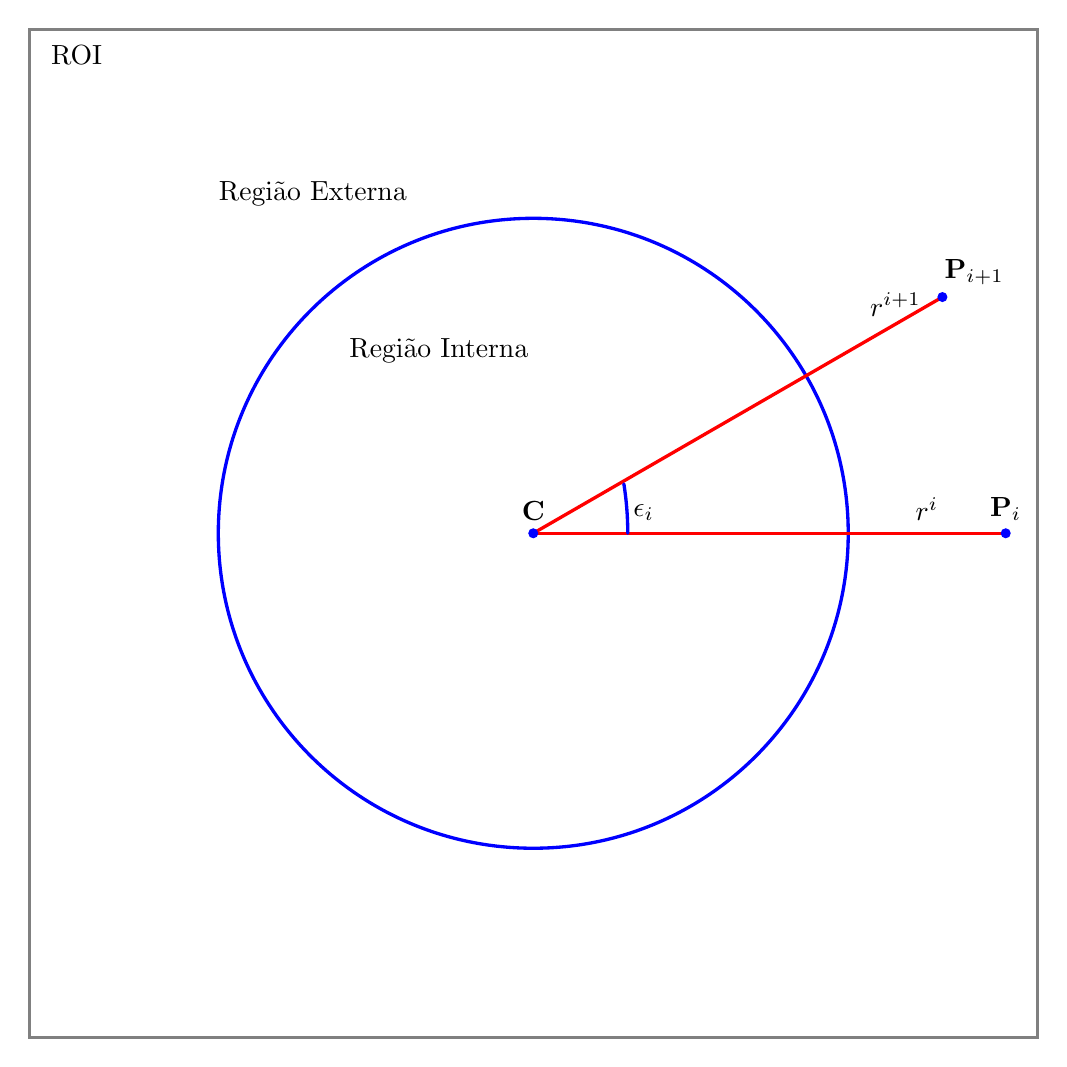
\begin{tikzpicture}[scale=4.0,cap=round,>=latex]
        \draw[blue, very thick] (0cm,0cm) circle(1cm);
        \draw[gray,  very thick] (-1.6,-1.6) rectangle (1.6,1.6);
        \foreach \x in {0,30} {
                \draw[red,  very thick] (0.0cm,0.0cm) -- (\x:1.5cm);
                \filldraw[blue] (\x:1.5cm) circle(0.4pt);
        }
        \draw (1.5cm,0cm) node[above=1pt] {$\mathbf{P}_i$};
        \draw (1.25cm,0cm) node[above=1pt] {$\bm{r}^i$};
        \draw (1.4cm,0.75cm) node[above=1pt] {$\mathbf{P}_{i+1}$};
        \draw (1.15cm,0.65cm) node[above=1pt] {$\bm{r}^{i+1}$};
        \draw (0cm,0cm) node[above=1pt] {$\mathbf{C}$};
        \filldraw[blue] (0cm,0cm) circle(0.4pt);
        \draw (-0.7cm,1cm) node[above=1pt] {Região Externa};
        \draw (-0.3cm,0.5cm) node[above=1pt] {Região Interna};
        \draw (-1.45cm,1.45cm) node[above=1pt] {ROI};
        \draw[blue,  very thick] (0.3cm,0) arc (0:9:1);
        \draw (0.35cm,0cm) node[above=1pt] {$\epsilon_i$};
    \end{tikzpicture}
	\caption{Definições para a ROI na imagem PolSAR.}
\label{fig:cap_det_bor_radiais}
\end{figure}

O algoritmo \textit{Bresenham's midpoint line} é usado para definir e extrair informações ao longo de cada linha radial. 

\subsection{Estimativa por máxima verossimilhança}\label{metodo_mle_est_param}

A técnica de máxima verossimilhança (MLE -- \textit{Maximum Likelihood Estimation}) permite estimar os parâmetros de um modelo estatístico usando uma amostra de dados observados.
Essa técnica é desejável por apresentar boas propriedades em relação a outras abordagens.

Suponha $\bm z = (z_1,\dots,z_n)$ um vetor de variáveis aleatórias independentes e identicamente distribuídas segundo uma distribuição caracterizada pela função de densidade de probabilidade $f(\bm z,\mathbf{\theta})$ que, por sua vez, é indexada pelos parâmetros $\mathbf{\theta}=(\theta_1,\dots,\theta_d)^T$ pertencentes ao espaço paramêtrico $\Theta$. 
Definimos, então a função de verossimilhança 
\begin{equation}\label{eq:funcao_de_verossimilhanca_theta}
   L(\theta;\bm z) = \prod_{k=1}^{n}f(z_k;\theta), 
\end{equation}
e a função log-verossimilhança  
\begin{equation}\label{eq:funcao_de_log_verossimilhanca_theta}
	\mathcal{L}(\theta;\bm z)= \ln L(\theta;\bm z)  = \sum_{k=1}^{n}\ln f(z_k;\theta).
\end{equation}

O vetor de parâmetros $\theta$ é estimado pelo vetor $\widehat{\theta}$ tal que $\mathcal{L}(\widehat{\theta};\bm z)\ge \mathcal{L}(\theta;\bm z)$ para todo $\theta$ no espaço dos parâmetros $\Theta$. A estimativa de máxima verossimilhança pode ser representada por 
\begin{equation}\label{eq:max_vetor_log_theta}
    \widehat{\theta}= \text{arg}\,\max\limits_{\theta\in\Theta}\mathcal{L}(\theta;\bm z),
\end{equation}
em que $\bm z$ agora denota as observações.

\subsection{A máxima verossimilhança usando os parâmetros estimados}\label{sec:sub:mle_param_estimados}

Cada linha radial $\bm z = (z_1,z_2,\dots,z_n)$ é particionada em duas amostras disjuntas na posição $j$,
$$
\bm z = (\underbrace{z_1,z_2,\dots,z_j}_{\bm z_\text{I}}, 
\underbrace{z_{j+1}, z_{j+2},\dots,z_n}_{\bm z_\text{E}}),
$$
para as quais são definidos modelos estatísticos diferentes, um modelo para
$\bm Z_\text{I} \sim W(\Sigma_\text{I},L_\text{I})$, e outro modelo para
$\bm Z_\text{E} \sim W(\Sigma_\text{E},L_\text{E})$.

O método MLE, descrito na seção \eqref{metodo_mle_est_param}, é aplicado nas amostras internas $\bm z_\text{I}$ e externas $\bm z_\text{E}$ para estimar $(\Sigma_\text{I},L_\text{I})$ e $(\Sigma_\text{E},L_\text{E})$ maximizando~\eqref{eq:funcao_de_log_verossimilhanca_theta}, e obtendo $(\widehat{\Sigma}_\text{I}, \widehat{L}_\text{I})$ e $(\widehat{\Sigma}_\text{E}, \widehat{L}_\text{E})$.

A função de verossimilhança é definida no ponto $j$ de acordo com a função
\begin{equation}\label{eq:vero_prod_int_ext}
	L(j; \bm z)=\prod_{k=1}^{j}f_{\mathbf{Z}}(\bm z_k;\mathbf{\Sigma}_k,L_k) \prod_{k=j+1}^{n}f_{\mathbf{Z}}(\bm z_k;\mathbf{\Sigma}_k,L_k).
\end{equation}

Usando propriedades de logaritmos naturais para cada termo do produtório \eqref{eq:vero_prod_int_ext} é definida a função log-verossimilhança total dependendo de $j$:
\begin{equation}\label{eq:log_vero_int_ext}
	\mathcal{L}(j)=\ln L(j)=\sum_{k=1}^{j}\ln f_{\mathbf{Z}}(\bm z_k;\mathbf{\Sigma}_k,L_k)+ \sum_{k=j+1}^{n}\ln f_{\mathbf{Z}}(\bm z_k;\mathbf{\Sigma}_k,L_k).
\end{equation}

O estimador de máxima verossimilhança $\widehat{\jmath}_{\text{ML}}$ é uma evidência de borda, pois representa uma aproximação da transição entre regiões, sendo
\begin{equation}\label{eq:max_j_ml}
\begin{array}{rcl}
	\widehat{\jmath}_{\text{ML}}&=&\text{arg}\max\limits_{j}\mathcal{L}(j).
\end{array}
\end{equation}
É importante destacar que os parâmetros a serem estimados em~\eqref{eq:max_j_ml} são os números de looks $L$ (do lado interno e do lado externo),
as matrizes de covariância $\mathbf\Sigma$ (do lado interno e do lado externo),
e o ponto $j$.
A evidência de borda é encontrada aplicando-se o método GenSA~\citep{xgsh}.

\section{O MLE para a distribuição gama}\label{sec:eml_pdf_gamma}

Cada canal de intensidade pode ser modelado por uma lei gama, como apresentado em~\eqref{pdf_inten_multilook}:
\begin{equation}\label{pdf_gauss_univ}
	f_{Z}(z;\mu,L)=\frac{L^{L}}{\Gamma(L)\mu^{L}} z^{L-1}\exp\left\{-\frac{L}{\mu}z\right\}, %\\ %%% ACF Não use quebra de linha a não ser que se trate de um empilhamento de equações
\end{equation}
onde, $\mu>0$ e $L>0$.
Aplicando o logaritmo natural obtemos:
\begin{equation}\nonumber
\begin{array}{ccl}
	\ln f_{Z}(z;\mu,L)&=&\ln \left(\frac{L^{L}}{\Gamma(L)\mu^{L}} z^{L-1}\exp\left\{-\frac{L}{\mu}z\right\}\right), \\
	                                         &=&\ln\left(\frac{L}{\mu}\right)^L-\ln\Gamma(L)+ \ln z^{L-1} + \ln \exp\left\{-L\frac{z}{\mu}\right\}, \\
%	                                         &=&L\ln\frac{L}{\mu}-\ln\Gamma(L)+(L-1)\ln z - \frac{L}{\mu} z,\\	                                         
\end{array}
\end{equation}
obtendo a função,
\begin{equation}\label{func_log_univ_gaussiana}
	\ln f_{Z}(z;\mu,L)=L\ln\frac{L}{\mu}-\ln\Gamma(L)+(L-1)\ln z - \frac{L}{\mu} z.
\end{equation}

Dada a amostra $\bm z = (z_1,\dots,z_n)$ extraída dos canais de intensidades hh, hv, e vv, é definida a função log-verossimilhança, como  
\begin{equation}\nonumber
\begin{split}
  \mathcal{L}(\bm z;\mu, L)=\ln\prod_{k=1}^{n}f_Z(z_k;\mu,L)\\
  \mathcal{L}(\bm z;\mu, L)=\sum_{k=1}^{n}\ln f_Z(z_k;\mu,L).
 \end{split}
 \end{equation}
 
Com o uso da função logarítmica~\eqref{func_log_univ_gaussiana}, teremos
\begin{equation}\nonumber
\begin{split}
    \mathcal{L}(\bm z;\mu, L)&=\sum_{k=1}^{n}\ln f_Z(z_k;\mu,L)\\
                      &=\sum_{k=1}^{n}\left[L\ln\frac{L}{\mu}-\ln\Gamma(L)+(L-1)\ln z_k - \frac{L}{\mu} z_k\right]\\
                      &=\sum_{k=1}^{n}L\ln\frac{L}{\mu}-\sum_{k=1}^{n}\ln\Gamma(L)+(L-1)\sum_{k=1}^{n}\ln z_k - \frac{L}{\mu}\sum_{k=1}^{n} z_k\\
                      &=L\ln\frac{L}{\mu}\sum_{k=1}^{n}1-\ln\Gamma(L)\sum_{k=1}^{n}1+(L-1)\sum_{k=1}^{n}\ln z_k - \frac{L}{\mu}\sum_{k=1}^{n} z_k\\
                      &=L\ln\frac{L}{\mu}n-\ln\Gamma(L)n+(L-1)\sum_{k=1}^{n}\ln z_k - \frac{L}{\mu}\sum_{k=1}^{n} z_k.              
 \end{split}
 \end{equation}

A função log-verossimilhança para a PDF univariada~\eqref{pdf_gauss_univ} pode ser reescrita por
\begin{equation}\nonumber
    \mathcal{L}(\bm z;\mu, L)=n\left[L\ln\frac{L}{\mu}-\ln\Gamma(L)\right]+(L-1)\sum_{k=1}^{n}\ln z_k - \frac{L}{\mu}\sum_{k=1}^{n} z_k,
 \end{equation}
e a sua forma reduzida, em que eliminamos os termos que não dependem dos parâmetros, por 
\begin{equation}
\mathcal{L}(\bm z;\mu, L) = 
n \left[L\ln \frac{L}{\mu} - \ln \Gamma(L)\right]
+L \sum_{k=1}^{n}\ln z_k -\frac{L}{\mu}\sum_{k=1}^{n} z_k.
\label{eq:LogLikelihoodGamma_red}
\end{equation}

A função~\eqref{eq:LogLikelihoodGamma_red} é usada para estimar os parâmetros $(\widehat \mu, \widehat L)$ com o método MLE de $(\mu, L)$ baseado na amostra $\bm z$. 
O ponto que maximiza a função~\eqref{eq:LogLikelihoodGamma_red} é encontrado com o método BFGS, implementado no pacote \texttt{maxLik} \citep{ht}. 
Para alcançar uma melhor estabilidade numérica, optou-se por realizar o processo de otimização resolvendo $\nabla\mathcal{L}=\bm 0$. 

De acordo com a seção \ref{sec:sub:mle_param_estimados} é extraído de cada canal de intensidade da imagem PolSAR uma faixa de dados $\bm z = (z_1,z_2,\dots,z_n)$ de forma que seja particionada em duas amostras, disjuntas, na posição $j$:  
$$
\bm z = (\underbrace{z_1,z_2,\dots,z_j}_{\bm z_\text{I}}, 
\underbrace{z_{j+1}, z_{j+2},\dots,z_n}_{\bm z_\text{E}}),
$$
para as quais são definidos modelos estatísticos diferentes, um modelo para
$\bm Z_\text{I} \sim \Gamma(\mu_\text{I},L_\text{I})$, e outro modelo para
$\bm Z_\text{E} \sim \Gamma(\mu_\text{E},L_\text{E})$.

As funções log-verossimilhança reduzidas aplicadas nas amostras internas $\bm z_\text{I}$ e externas $\bm z_\text{E}$ são usadas para estimar os parâmetros $(\mu_\text{I},L_\text{I})$ e $(\mu_\text{E},L_\text{E})$ maximizando~\eqref{eq:LogLikelihoodGamma_red}, e obtendo $(\widehat{\mu}_\text{I}, \widehat{L}_\text{I})$ e $(\widehat{\mu}_\text{E}, \widehat{L}_\text{E})$.


A log-verossimilhança total é definida no ponto $j$ pela seguinte função
\begin{equation}\label{eq:TotalLogLikelihood}
\begin{split}
%\ell(j&;\bm z_\text{I},\bm z_\text{E}) = \\
\ell(j&;\widehat{\mu}_I, \widehat{L}_I,\widehat{\mu}_E, \widehat{L}_E)=\\
&j \big[\widehat{L}_\text{I}\ln (\widehat{L}_\text{I} / \widehat{\mu}_\text{I}) - \ln \Gamma(\widehat{L}_\text{I})\big]
+\widehat{L}_\text{I} \sum_{k=1}^{j}\ln z_k -\frac{\widehat{L}_\text{I}}{\widehat{\mu}_\text{I}}\sum_{k=1}^{j} z_k +\\
&(n-j) \big[\widehat{L}_\text{E}\ln (\widehat{L}_\text{E} / \widehat{\mu}_\text{E}) - \ln \Gamma(\widehat{L}_\text{E})\big]
+\widehat{L}_\text{E} \sum_{k=j+1}^{n}\ln z_k - \frac{\widehat{L}_\text{E}}{\widehat{\mu}_\text{E}}\sum_{k=j+1}^{n} z_k,
\raisetag{2.2em}
\end{split}
\end{equation}
e aplicando o método GenSA~\citep{xgsh} encontramos a evidência de borda
$$
\widehat{\jmath}= \arg\max\limits_{j\in [\min_s,N-\min_s]}\ell(j;\widehat{\mu}_I, \widehat{L}_I,\widehat{\mu}_E, \widehat{L}_E),
$$ 
onde $\min_s$ é uma constante de folga mínima definida empiricamente para as extremidades da amostra. A escolha do número de píxeis da amostra pode variar de acordo com a ROI, com o canal, ou com o tipo de sensor para aquisição de imagem.
